%%%%%%%%%%%%%%%%%%%%%%%%%%%%%%%%%%%%
\justifying
\section{6.6. Inferência para diferença entre duas proporções com uma amostra pequena}

%%%%%%%%%%%%%%%%%%%%%%%%%%%%%%%%%%%%

\begin{frame}
\frametitle{Comparando as costas da mão à palma da mão}
\justifying
MythBusters também pediu a essas pessoas para adivinharem as palmas das mãos. Desta vez, 7 das 12 pessoas acertaram. Os dados estão resumidos abaixo.

\begin{center}
\begin{tabular}{ l | c | c | c }
          & Dorso		& Palma		& Total \\
\hline
Correto		& 11			& 7				& 18 \\
Errado		  & 1				& 5				& 6 \\
\hline
Total			& 12			& 12			& 24 \\
\end{tabular}
\end{center}

\end{frame}

%%%%%%%%%%%%%%%%%%%%%%%%%%%%%%%%%%%%

\begin{frame}
\frametitle{Proporção de palpites corretos}

{\small
\begin{center}
\begin{tabular}{ l | c | c | c }
          & Dorso  	& Palma		& Total \\
\hline
Correto		& 11			& 7				& 18 \\
Errado		  & 1				& 5				& 6 \\
\hline
Total			& 12			& 12			& 24 \\
\end{tabular}
\end{center}

}

\begin{itemize}
\justifying
\item Proporção de acertos no grupo do dorso: $\frac{11}{12} = 0.916$
\justifying
\item Proporção de correto no grupo da palme: $\frac{7}{12} = 0.583$
\justifying
\item Diferença: 33.3\% mais acertos do grupo que avaliou o dorso das mãos.

\end{itemize}
\justifying
\dq{Com base nas proporções calculadas, você acha que a chance de adivinhar corretamente o dorso da mão é diferente da palma da mão?}

\end{frame}

%%%%%%%%%%%%%%%%%%%%%%%%%%%%%%%%%%%%

\begin{frame}
\frametitle{Hipóteses}
\justifying
\dq{Quais são as hipóteses para comparar se a proporção de pessoas que conseguem adivinhar corretamente o dorso de suas mãos é diferente da proporção de pessoas que conseguem adivinhar corretamente a palma de suas mãos?}

\begin{itemize}
\item[$H_0$:] $p_{dorso} = p_{palma}$
\item[$H_0$:] $p_{dorso} \ne p_{palma}$
\end{itemize}

\end{frame}

%%%%%%%%%%%%%%%%%%%%%%%%%%%%%%%%%%%%

\begin{frame}
\frametitle{Condições?}

\begin{itemize}
\justifying
\item Independência - dentro de grupos, entre grupos?
\begin{itemize}
\justifying
\item Dentro de cada grupo podemos supor que o palpite de um sujeito é independente do outro.
\justifying
\item Entre os grupos, a independência não é satisfeita - temos as mesmas pessoas adivinhando. No entanto, vamos supor que são suposições independentes para continuar com a análise.
\end{itemize}
\justifying
\item Tamanho da amostra?
\begin{itemize}
\justifying
\item $\hat{p}_{amostra} = \frac{11 + 7}{12 + 12} = \frac{18}{24} = 0.75$.
\justifying
\item Sucessos esperados no grupo do dorso: $ 12 \times 0.75 = 9 $, falhas = 3.
\justifying
\item Sucessos esperados no grupo da palma: $ 12 \times 0.75 = 9 $, falhas = 3.
\justifying
\item Como a condição Sucessos/Fracassos falha, precisamos usar a simulação para comparar as proporções.
\end{itemize}

\end{itemize}

\end{frame}

%%%%%%%%%%%%%%%%%%%%%%%%%%%%%%%%%%%%

\subsection{Aleatorização HT para comparar duas proporções}

%%%%%%%%%%%%%%%%%%%%%%%%%%%%%%%%%%%%

\begin{frame}
\frametitle{Esquema de simulação}

\begin{enumerate}
\justifying
\item Use 24 fichas de índice, onde cada cartão representa um assunto.
\justifying
\item Marque 18 das cartas como "corretas" e as 6 restantes como "erradas".
\justifying
\item Embaralhe as cartas e divida em dois grupos de tamanho 12, para as costas e a palma da mão.
\justifying
\item Calcule a diferença entre as proporções de "correto para o dorso" e nos decks de palma, e registre este número.
\justifying
\item Repita as etapas (3) e (4) várias vezes para criar uma distribuição aleatória das diferenças nas proporções simuladas.

\end{enumerate}

\end{frame}

%%%%%%%%%%%%%%%%%%%%%%%%%%%%%%%%%%%%

\begin{frame}
\frametitle{Interpretando os resultados da simulação}
\justifying
Simulando o experimento sob o pressuposto de independência, ou seja, deixando as coisas ao acaso. \\

\vspace{0.5cm}
\justifying
Se os resultados das simulações baseadas no modelo nulo se parecem com os dados, então podemos determinar que a diferença entre as proporções das estimativas corretas nos dois grupos foi simplesmente \hl{devido ao acaso}. \\

\vspace{0.5cm}
\justifying
Se os resultados das simulações baseadas no modelo nulo não se parecem com os dados, então podemos determinar que a diferença entre as proporções dos palpites corretos nos dois grupos não foi devida ao acaso, mas \hl{sim porque as pessoas realmente conhecem o dorso de suas mãos melhor do que a palma}.

\end{frame}

%%%%%%%%%%%%%%%%%%%%%%%%%%%%%%%%%%%%

\begin{frame}
\frametitle{Resultados simulados}

\begin{itemize}
\justifying
\item No próximo slide você pode ver o resultado de um teste de hipótese (usando apenas 100 simulações para manter os resultados simples).
\justifying
\item Cada ponto representa uma diferença na proporção simulada de sucessos. Podemos ver que a distribuição está centrada em 0 (o valor nulo).
\justifying
\item Também podemos ver que 9 das 100 simulações produziram diferenças simuladas pelo menos tão grandes quanto a diferença observada (p-valor = 0.09).

\end{itemize}

\end{frame}

%%%%%%%%%%%%%%%%%%%%%%%%%%%%%%%%%%%%

\begin{frame}[fragile]
\frametitle{Simulação}

{\tiny
\begin{Verbatim}[frame=single, formatcom=\color{blue}]
mão = as.factor (c (rep ("correto", 7), rep ("errado", 5), c (rep ("correto", 11), rep ("errado", 1))))
gr = c(rep("palma",12),rep("dorso",12))
inferência (mão, gr, est = "proporção", tipo = "ht", null = 0, alternativa = "twosided",
	order = c ("voltar", "palma"), sucesso = "correto", método = "simulação", semente = 879,
	nsim = 100)
\end{Verbatim}
}

\pause

{\tiny
\begin{Verbatim}[frame=single, formatcom=\color{gray}]
Variável de resposta: categórica, Variável explicativa: categórica
Diferença entre duas proporções - sucesso: correto
Estatísticas resumidas:
         x
y         soma  palma  dorso
  correto   11    7  18
  errado      1    5   6
  soma       12   12  24
Diferença observada entre proporções (palma da mão) = 0.3333
H0: dorso - p_palma = 0 
HA: p_dorso - p_palma != 0 
valor-p =  0.18 
\end{Verbatim}
}

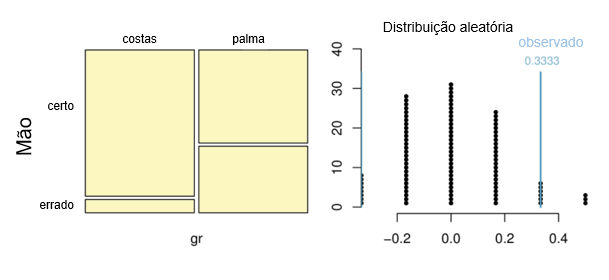
\includegraphics[width=0.8\textwidth,height=0.3\textheight]{6-6_small_two_props/palm_back_HT.png}

\end{frame}

%%%%%%%%%%%%%%%%%%%%%%%%%%%%%%%%%%%

\begin{frame}
\frametitle{Conclusão}
\justifying
\pq{Os resultados da simulação sugerem que as pessoas conhecem melhor o dorso das mãos do que a palma? \\
(Lembre-se: havia 33.3 \% mais acertos no grupo ddo dorso nos dados observados.)}

\begin{enumerate}[(a)]
\item Sim
\solnMult{Não}
\end{enumerate}
\justifying
p-valor = 0.09 $>$ 0.05, não rejeitar $H_0$. Os dados não fornecem evidências convincentes de que as pessoas conhecem melhor o dorso das mãos do que a palma das mãos.

\end{frame}

%%%%%%%%%%%%%%%%%%%%%%%%%%%%%%%%%%%%%